\documentclass[a4paper,10pt]{article} 
\usepackage[utf8]{inputenc}
\usepackage[a4paper]{geometry}
\usepackage[magyar]{babel}
\usepackage{amsmath}
\usepackage{amssymb}
\usepackage{pgf,tikz}
\usetikzlibrary{arrows}
\usepackage{caption}
\frenchspacing 
\pagestyle{empty}
\newcommand{\ki}[2]{\hfill {\it #1 (#2)}\medskip}
\newcommand{\vonal}{\hbox to \hsize{\hskip2truecm\hrulefill\hskip2truecm}}
\newcommand{\degre}{\ensuremath{^\circ}}
\newcommand{\tg}{\mathop{\mathrm{tg}}\nolimits}
\newcommand{\ctg}{\mathop{\mathrm{ctg}}\nolimits}
\newcommand{\arc}{\mathop{\mathrm{arc}}\nolimits}
\begin{document}
\begin{center} \Large {\em XXI. Nemzetközi Magyar Matematika Verseny} \end{center}
\begin{center} \large{\em Kecskemét, 2012. március 14--18.} \end{center}
\smallskip
\begin{center} \large{\bf 10. osztály} \end{center}
\bigskip 

{\bf 1. feladat: } Van-e olyan egész együtthatós $P(x)$ polinom, amelyre 
$P(0)=12, P(1)=20$ és $P(2)=2012$?

\ki{Pintér Ferenc}{Nagykanizsa}\medskip

{\bf Megoldás: } Mivel a polinom három helyettesítési értéke adott, vizsgáljuk meg, hogy létezik-e megfelelő másodfokú polinom; ha van, akkor az egyértelmű. Az egyszerűbb számolás
végett keressük a polinomot
\[P(x)=ax(x-1)+bx+c\]
alakban! (Így az $x=1$ helyettesítés egyszerűbb egyenletet fog eredményezni.)

Ekkor
\begin{align}
\label{1}P(0)&=c=12\\
\label{2}P(1)&=b+c=20\\
\label{3}P(2)&=2a+2b+c=2012
\end{align}
\eqref{1} és \eqref{2} összevetésével $b=8$; a két másik együttható ismeretében \eqref{3}-ból $a=992$.

Így a $P(x)=992x(x-1)+8x+12=992x^2-984x+12$ megfelel a feltételeknek. Ezzel a feladat kérdését megválaszoltuk.

{\it Megjegyzés.} Természetesen vannak megfelelő magasabb fokszámú polinomok is. Egy ilyen
harmadfokú polinom például a $P(x)=330x^3+2x^2-324x+12$.

\medskip

\vonal
{\bf 2. feladat: } Határozzuk meg mindazokat a $p$, $q$, $r$ prímszámokat, amelyekre
\[pqr < pq + qr + rp\, !\]

\ki{Oláh György}{Révkomárom}\medskip

{\bf Megoldás: } A bizonyítandó egyenlőtlenség mindkét oldalát osszuk el a pozitív $pqr$ szorzattal:
\[\frac{pq+qr+rp}{pqr}=\frac{1}{p}+\frac{1}{q}+\frac{1}{r}>1.\]

Nem megy az általánosság rovására, ha feltételezzük, hogy $p\le q\le r$.

Ha $p=q=2$, akkor $r$ tetszőleges prímszám lehet, azaz ekkor végtelen sok megfelelő
rendezett prímhármas van.

Ha $p=2$, $q=3$, akkor $\frac{1}{r}>\frac16$, aminek $r=3$ és $r=5$ felelnek meg.

Ha $p=2$, $q>3$, akkor $\frac{3}{10}<\frac1r\le\frac15$, ami ellentmondás, tehát ekkor nincs megoldás.

Ha $p\ge 3$, akkor $\frac1p+\frac1q+\frac1r\le1$, azaz ebben az esetben sincs megoldás.

Összefoglalva a megoldások: $(2;2;r)$ ($r$ tetszőleges prím), $(2;3;3)$, $(2;3;5)$. Mivel a feltételben $p$, $q$ és $r$ szerepe azonos, ezen hármasok bármely permutációja megoldás.

\medskip

\vonal
{\bf 3. feladat: } Mely $n$ pozitív egész számok esetén lesz az $n^2+n+19$ kifejezés értéke négyzetszám?

\ki{Kacsó Ferenc}{Marosvásárhely}\medskip

{\bf I. megoldás: } Legyen
\begin{equation}
n^2+n+19=m^2,\label{4}
\end{equation}
ahol $m$ pozitív egész szám! Szorozzuk meg a \eqref{4} egyenlet mindkét oldalát 4-gyel, majd végezzünk átalakításokat.
\begin{align*}
4n^2+4n+76&=4m^2\\
(2m)^2-(2n+1)^2&=75\\
(2m-2n-1)(2m+2n+1)&=75
\end{align*}

Legyen
\begin{equation}
2m-2n-1=a\quad\text{és}\quad 2m+2n+1=b,\label{5}
\end{equation}
ahol $0<a<b$ egészek, és
\begin{equation}
ab=75\label{6}
\end{equation}
Az \eqref{5} egyenletrendszer megoldása $n$-re és $m$-re:
\[n=\frac{b-a-2}{4},\quad m=\frac{a+b}{4}.\]

A \eqref{6} feltételnek megfelelő $(a;b)$ párok: $(1;75)$, $(3;25)$, $(5;15)$. Ennek megfelelően a \eqref{4} egyenlet megoldásai a következő $(n;m)$ számpárok: $(18;19)$, $(5;7)$, $(2;5)$.

Az adott kifejezés tehát $n=2$, $n=5$ és $n=18$ esetén vesz fel négyzetszám értéket.

\medskip

{\bf II. megoldás: } Mivel $n^2+n+19>n^2$, a következő egyenletet kell megoldanunk:
\begin{equation}
n^2+n+19=(n+k)^2,\label{7}
\end{equation}
ahol $k$ pozitív egész szám.

A \eqref{7} egyenletet átalakítva:
\[19-k^2=n(2k-1).\]
Mivel $19-k^2>0$, ezért $k$ lehetséges értékei 1, 2, 3 és 4.

$k=1$-re $n=18$, $k=2$-re $n=5$, $k=3$-ra $n=2$. $k=4$ esetén $n$-re nincs pozitív egész megoldás.

Az adott kifejezés tehát $n=2$, $n=5$ és $n=18$ esetén vesz fel négyzetszám értéket.

\medskip

\vonal
{\bf 4. feladat: } Határozzuk meg az
\[E=\frac{2x}{3y+4z}+\frac{3y}{4z+2x}+\frac{4z}{2x+3y}\]
kifejezés legkisebb értékét, ha $x$, $y$ és $z$ pozitív valós számok!

\ki{Kovács Béla}{Szatmárnémeti}\medskip

{\bf I. megoldás: } Legyen $3y+4z=a$, $4z+2x=b$, $2x+3y=c$.

Ekkor
\[x=\frac{b+c-a}{4},\quad y=\frac{c+a-b}{6},\quad z=\frac{a+b-c}{8}\]
és
\[E=\frac{b+c-a}{2a}+\frac{c+a-b}{2b}+\frac{a+b-c}{2c}.\]

Alakítsuk és becsüljük $E$-t. Felhasználjuk, hogy pozitív szám és reciprokának összege legalább 2, és pontosan akkor 2, ha a szám az 1.
\begin{align*}
E&=\frac12\left(\frac{b}{a}+\frac{c}{a}-1+\frac{c}{b}+\frac{a}{b}-1+\frac{a}{c}+\frac{b}{c}-1\right)\\
&=\frac12\left(\left(\frac{a}{b}+\frac{b}{a}\right)+\left(\frac{b}{c}+\frac{c}{b}\right)+\left(\frac{c}{a}+\frac{a}{c}\right)-3\right)\ge\frac12(2+2+2-3)=\frac32
\end{align*}

$E$ legkisebb értéke tehát $\frac32$, és ezt akkor veszi fel, ha $a=b=c$, vagyis ha $2x=3y=4z$, ami azt jelenti, hogy az $x$, $y$, $z$ számok fordított arányban állnak a 2, 3, 4 számokkal.

\medskip

{\bf II. megoldás: } Legyen $a=2x$, $b=3y$, $c=4z$. Ezzel
\[E=\frac{a}{b+c}+\frac{b}{a+c}+\frac{c}{a+b}.\]
Ha $b+c=p$, $a+c=q$, $a+b=r$, akkor
\[E=\frac{q+r-p}{2p}+\frac{r+p-q}{2q}+\frac{p+q-r}{2r}.\]

Ez pontosan az I. megoldásban bemutatott alak, amelyről az ott leírt módon belátható, hogy minimuma $\frac{3}{2}$, és ezt akkor veszi fel, ha $p=q=r$, vagyis ha $b+c=a+c=a+b$, azaz $a=b=c$, tehát $2x=3y=4z$, ami azt jelenti, hogy az $x$, $y$, $z$ számok fordított arányban állnak a 2, 3, 4 számokkal.

\medskip

{\it Megjegyzés.} Az egyenlőtlenség $2x=a$, $3y=b$, $4z=c$ alakban Nesbitt-egyenlőtlenség néven ismert.

\medskip

\vonal
{\bf 5. feladat: } Az $ABC$ egyenlő szárú háromszögben $AC=BC$, 
az $AB$ alap felezőpontja $D$, az $A$ és a $D$ pontból
a $BC$ szakaszra bocsátott merőlegesek talppontja rendre a $BC$ szakasz $E$, illetve $F$ belső pontja. A $DF$ szakasz $G$ felezőpontját a $C$ ponttal összekötő szakasz és az $AF$ szakasz metszéspontja $H$.
Igazoljuk, hogy a $H$ pont az $AC$ szakasz mint átmérő fölé írt Thalész-körön van!

\ki{Bíró Bálint}{Eger}\medskip

{\bf Megoldás: } A $DF$ és $AE$ egyenesek párhuzamosak, hiszen mindkettő merőleges $BC$-re, és mivel $D$ az $AB$ oldal felezőpontja, $DF$ középvonal az $ABE$ háromszögben, így $F$ felezőpontja az $EB$ szakasznak. A $ABE\triangle$ és a $DBF\triangle$ háromszögek hasonlók, a hasonlóság aránya $2:1$.

A $DF$ szakasz a $BCD$ derékszögű háromszög átfogójához tartozó magassága, ez pedig -- mint ismeretes -- két hasonló háromszögre bontja a $BCD\triangle$-et, tehát $DBF\triangle\sim CDF\triangle$.

\begin{figure}
\begin{center}
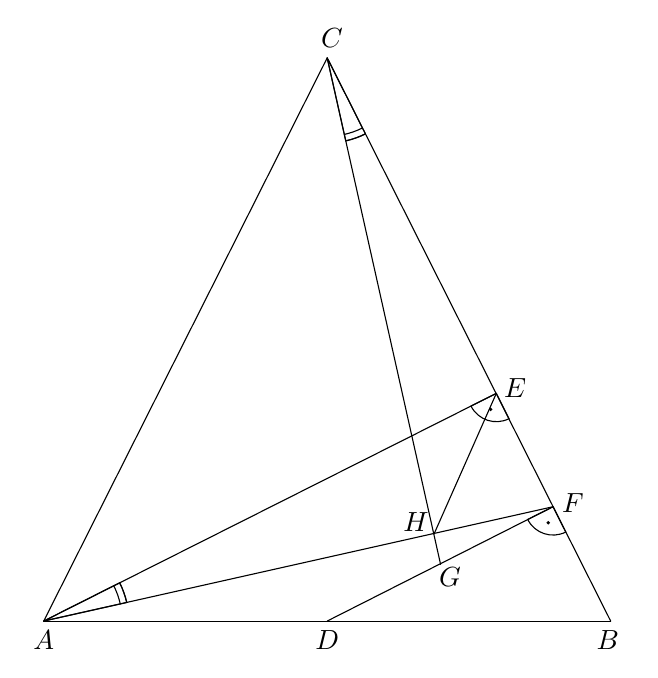
\begin{tikzpicture}[line cap=round,line join=round,>=triangle 45,x=1.2cm,y=1.2cm]
\clip(-3.17,-0.3) rectangle (3.2,6.28);
\draw [shift={(1.79,2.41)}] (0,0) -- (-153.27:0.3) arc (-153.27:-63.27:0.3) -- cycle;
\draw [shift={(2.39,1.21)}] (0,0) -- (-153.27:0.3) arc (-153.27:-63.27:0.3) -- cycle;
\draw [shift={(0,5.96)}] (0,0) -- (-77.4:0.9) arc (-77.4:-63.27:0.9) -- cycle;
\draw [shift={(-3,0)}] (0,0) -- (12.6:0.9) arc (12.6:26.73:0.9) -- cycle;
\draw (3,0)-- (0,5.96);
\draw (-3,0)-- (0,5.96);
\draw (-3,0)-- (3,0);
\draw (-3,0)-- (1.79,2.41);
\draw (0,0)-- (2.39,1.21);
\draw (-3,0)-- (2.39,1.21);
\draw (0,5.96)-- (1.2,0.6);
\fill(1.73,2.24) circle (0.02);
\fill(2.34,1.04) circle (0.02);
\draw [shift={(0,5.96)}] (-77.4:0.9) arc (-77.4:-63.27:0.9);
\draw [shift={(0,5.96)}] (-77.4:0.83) arc (-77.4:-63.27:0.83);
\draw [shift={(-3,0)}] (12.6:0.9) arc (12.6:26.73:0.9);
\draw [shift={(-3,0)}] (12.6:0.83) arc (12.6:26.73:0.83);
\draw (1.79,2.41)-- (1.13,0.92);
%\begin{scriptsize}
%\draw [fill=black] (-3,0) circle (1.5pt);
\draw[color=black] (-3,-0.2) node {$A$};
%\draw [fill=black] (3,0) circle (1.5pt);
\draw[color=black] (2.97,-0.2) node {$B$};
%\draw [fill=black] (0,5.96) circle (1.5pt);
\draw[color=black] (0.05,6.17) node {$C$};
%\draw [fill=black] (0,0) circle (1.5pt);
\draw[color=black] (-0.0,-0.2) node {$D$};
%\draw [fill=black] (1.79,2.41) circle (1.5pt);
\draw[color=black] (1.99,2.47) node {$E$};
%\draw [fill=black] (2.39,1.21) circle (1.5pt);
\draw[color=black] (2.6,1.25) node {$F$};
%\draw [fill=black] (1.2,0.6) circle (1.5pt);
\draw[color=black] (1.3,0.47) node {$G$};
%\draw [fill=black] (1.13,0.92) circle (1.5pt);
\draw[color=black] (0.94,1.05) node {$H$};
%\end{scriptsize}
\end{tikzpicture}
\end{center}
\caption*{Az 5. feladathoz.}
\end{figure}

A hasonlóság tranzitivitása miatt $ABE\triangle\sim CDF\triangle$, a megfelelő oldalak aránya tehát egyenlő:
\[\frac{AE}{EB}=\frac{CF}{FD}.\]

Mivel $FD=2FG$ és $EB=2EF$, ezért
\begin{equation}
\frac{AE}{EF}=\frac{CF}{FG}\label{8}
\end{equation}

A \eqref{8} egyenlőség szerint $AEF\triangle$ és $CFG\triangle$ két-két oldalának aránya megegyezik, és mivel ezen háromszögekben az $E$, illetve az $F$ csúcsnál derékszög van, a két háromszög hasonló.

Emiatt a megfelelő szögek egyenlők, tehát $FAE\sphericalangle=GCF\sphericalangle=HCF\sphericalangle$.

Az $A$ és $C$ pontok az $EH$ egyenes azonos oldalán vannak (mert $H$ és $C$ az $AE$ egyenes különböző oldalain vannak), az előzőek szerint pedig az $A$ és $C$ pontokból az $EH$ szakasz egyenlő nagyságú szögben látszik, így az $A$, $H$, $E$ és $C$ pontok egy körre illeszkednek. Mivel az $AEC$ háromszög derékszögű, ezért ez a kör az $AC$ szakasz Thalész-köre (azaz az $AH$ és $CH$, vagyis az $AF$ és $CG$ egyenesek merőlegesek).

Ezzel a feladat állítását igazoltuk.

\medskip

\vonal
{\bf 6. feladat: } Az első 2012 darab pozitív egész szám mindegyikét átírjuk hármas számrendszerbe. Hány palindrom szám van a kapott 2012 darab hármas számrendszerbeli szám között? (Palindrom számon
olyan pozitív egész számot értünk, amelynek számjegyeit fordított sorrendben írva az eredeti
számot kapjuk vissza.)

\ki{Kosztolányi József}{Szeged}\medskip

{\bf Megoldás: } Mivel $3^6=729<2012<2187=3^7$, ezért a vizsgált pozitív egészek a hármat számrendszerben legfeljebb hétjegyűek.

Két egyjegyű palindrom van: az 1 és a 2. Kétjegyűből is kettő van: 11 és 22.

Ha $n\ge1$, akkor a $2n$ jegyű hármas számrendszerbeli palindrom számokból úgy kapjuk a $2n+1$ jegyű palindrom számokat, hogy az első $n$ jegy után (középre) beírjuk a 0, 1, 2 számjegyek valamelyikét.

A $2n$ jegyű hármas számrendszerbeli palindrom számokból hasonlóan kapjuk a $2n+2$ jegyű palindrom számokat is: itt 00-t, 11-et vagy 22-t írunk be középre.

Ezek alapján Háromjegyű és négyjegyű palindrom számokból is 6 darab van, öt- és hatjegyűből 18, hétjegyűből pedig 54 darab.

Mivel $2012=2202112$, ezért a hétjegyű palindrom számok közül az ennél nagyobbak már nincsenek benne az alaphalmazban, ez összesen 6 darab szám: $2210122$, $2211122$, $2212122$, $2220222$, $2221222$, $2222222$.

Így az első 2012 darab pozitív egész közül a hármas számrendszerben palindromok száma: $2+2+6+6+18+18+54-6=100$.

\end{document}